\chapter{結果}

\begin{comment}
\begin{figure*}[h]
  \begin{center}
    \begin{tabular}{c}

      % 1
      \begin{minipage}[b]{0.3\linewidth}
        \begin{center}
          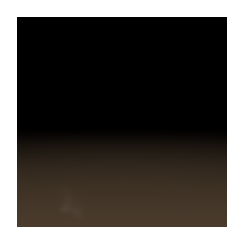
\includegraphics{./img/steam3d/render_50.eps}
        \end{center}
        \subcaption{50タイムステップ後}
      \end{minipage}

      % 2
      \begin{minipage}[b]{0.3\linewidth}
        \begin{center}
          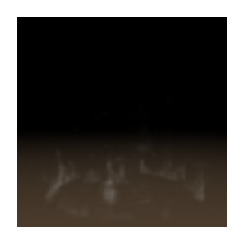
\includegraphics{./img/steam3d/render_100.eps}
        \end{center}
        \subcaption{100タイムステップ後}
      \end{minipage}
      
      % 3
      \begin{minipage}[b]{0.3\linewidth}
        \begin{center}
          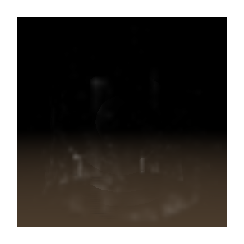
\includegraphics{./img/steam3d/render_150.eps}
        \end{center}
        \subcaption{150タイムステップ後}
      \end{minipage}
      \\\\
      % 4
      \begin{minipage}[b]{0.3\linewidth}
        \begin{center}
          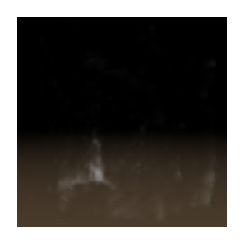
\includegraphics{./img/steam3d/render_200.eps}
        \end{center}
        \subcaption{200タイムステップ後}
      \end{minipage}

      % 5
      \begin{minipage}[b]{0.3\linewidth}
        \begin{center}
          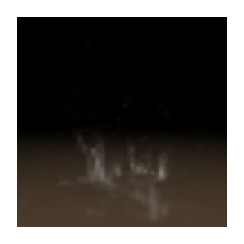
\includegraphics{./img/steam3d/render_250.eps}
        \end{center}
        \subcaption{250タイムステップ後}
      \end{minipage}

      % 6
      \begin{minipage}[b]{0.3\linewidth}
        \begin{center}
          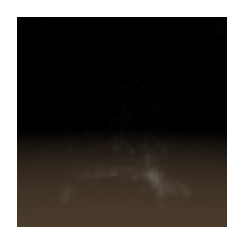
\includegraphics{./img/steam3d/render_300.eps}
        \end{center}
        \subcaption{300タイムステップ後}
      \end{minipage}
      \\\\

      % 7
      \begin{minipage}[b]{0.3\linewidth}
        \begin{center}
          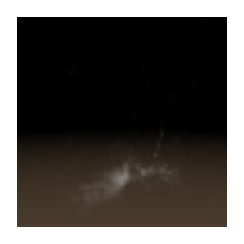
\includegraphics{./img/steam3d/render_350.eps}
        \end{center}
        \subcaption{350タイムステップ後}
      \end{minipage}

      % 8
      \begin{minipage}[b]{0.3\linewidth}
        \begin{center}
          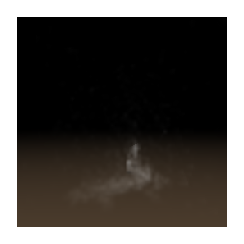
\includegraphics{./img/steam3d/render_400.eps}
        \end{center}
        \subcaption{400タイムステップ後}
      \end{minipage}

      % 9
      \begin{minipage}[b]{0.3\linewidth}
        \begin{center}
          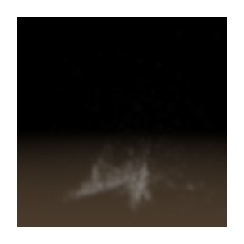
\includegraphics{./img/steam3d/render_450.eps}
        \end{center}
        \subcaption{450タイムステップ後}
      \end{minipage}

    \end{tabular}
    \caption{湯気のシミュレーションのレンダリング結果}
    \label{result}
  \end{center}
\end{figure*}

湯気のシミュレーションのレンダリング結果を図(\ref{result})に示す.
レンダリングは格子ごとに湯気の密度を合計し,ボリュームレイキャスティング法により行った.
シミュレーション空間は32×32×32の格子で,底辺の温度と水蒸気量はパーリンノイズを加えている.
シミュレーションで発生した粒子数は3,000個から6,000個となった.
計算時間はIntel Core i5-6200U 2.3GHzのCPUを用いて1タイムステップあたり3秒から4秒となった.

本手法により底面から湯気が発生し消滅する様子を再現した.
問題点としてタイムステップ数が大きくなるごとに流体全体が大きな渦を発生させる現象が発生することにより,湯気も安定した形を保つことができないことがあげられる.図(\ref{result})のレンダリング結果では300タイムステップ以降に偏りのある形となっている.原因としては流体の密度が小さいことでベナール対流と呼ばれる大きな渦の形を形成するためである.

\begin{figure*}[h]
  \begin{center}
    \begin{tabular}{c}

      % 1
      \begin{minipage}[b]{0.3\linewidth}
        \begin{center}
          
\includegraphics{./img/steam3d-highdens/render_50.eps}
        \end{center}
        \subcaption{50タイムステップ後}
      \end{minipage}

      % 2
      \begin{minipage}[b]{0.3\linewidth}
        \begin{center}
          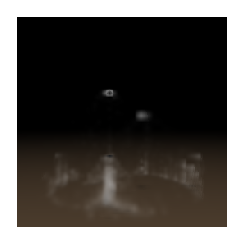
\includegraphics{./img/steam3d-highdens/render_100.eps}
        \end{center}
        \subcaption{100タイムステップ後}
      \end{minipage}
      
      % 3
      \begin{minipage}[b]{0.3\linewidth}
        \begin{center}
          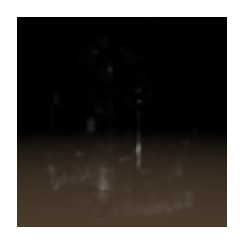
\includegraphics{./img/steam3d-highdens/render_150.eps}
        \end{center}
        \subcaption{150タイムステップ後}
      \end{minipage}
      \\\\
      % 4
      \begin{minipage}[b]{0.3\linewidth}
        \begin{center}
          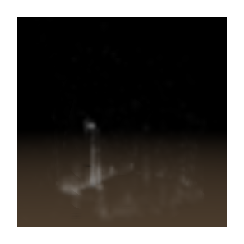
\includegraphics{./img/steam3d-highdens/render_200.eps}
        \end{center}
        \subcaption{200タイムステップ後}
      \end{minipage}

      % 5
      \begin{minipage}[b]{0.3\linewidth}
        \begin{center}
          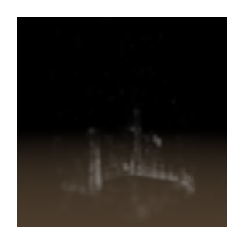
\includegraphics{./img/steam3d-highdens/render_250.eps}
        \end{center}
        \subcaption{250タイムステップ後}
      \end{minipage}

      % 6
      \begin{minipage}[b]{0.3\linewidth}
        \begin{center}
          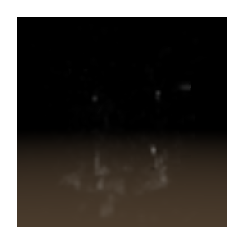
\includegraphics{./img/steam3d-highdens/render_300.eps}
        \end{center}
        \subcaption{300タイムステップ後}
      \end{minipage}
      \\\\

      % 7
      \begin{minipage}[b]{0.3\linewidth}
        \begin{center}
          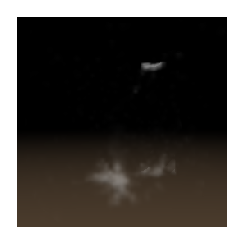
\includegraphics{./img/steam3d-highdens/render_350.eps}
        \end{center}
        \subcaption{350タイムステップ後}
      \end{minipage}

      % 8
      \begin{minipage}[b]{0.3\linewidth}
        \begin{center}
          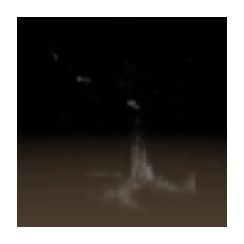
\includegraphics{./img/steam3d-highdens/render_400.eps}
        \end{center}
        \subcaption{400タイムステップ後}
      \end{minipage}

      % 9
      \begin{minipage}[b]{0.3\linewidth}
        \begin{center}
          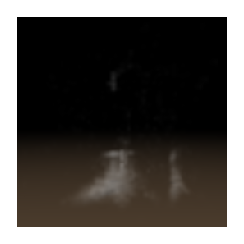
\includegraphics{./img/steam3d-highdens/render_450.eps}
        \end{center}
        \subcaption{450タイムステップ後}
      \end{minipage}

    \end{tabular}
    \caption{湯気のシミュレーションのレンダリング結果(流体の密度を高くした場合)}
    \label{result-high_dens}
  \end{center}
\end{figure*}

流体の密度を高くしたレンダリング結果を図(\ref{result-high_dens})に示す.
この場合,湯気が立ち上る量が多くなり,500タイムステップ以降も湯気の形状が偏りを発生することがないことを確認した.


\begin{figure*}[h]
  \begin{center}
    \begin{tabular}{c}

      % 1
      \begin{minipage}[b]{0.3\linewidth}
        \begin{center}
          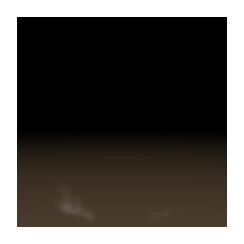
\includegraphics{./img/steam3d-highvapor/render_50.eps}
        \end{center}
        \subcaption{50タイムステップ後}
      \end{minipage}

      % 2
      \begin{minipage}[b]{0.3\linewidth}
        \begin{center}
          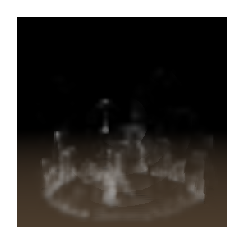
\includegraphics{./img/steam3d-highvapor/render_100.eps}
        \end{center}
        \subcaption{100タイムステップ後}
      \end{minipage}
      
      % 3
      \begin{minipage}[b]{0.3\linewidth}
        \begin{center}
          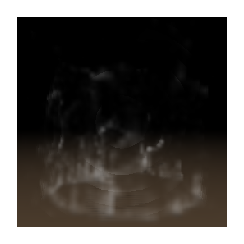
\includegraphics{./img/steam3d-highvapor/render_150.eps}
        \end{center}
        \subcaption{150タイムステップ後}
      \end{minipage}

    \caption{湯気のシミュレーションのレンダリング結果(蒸気量が多い場合)}
    \label{result-high_vapor}
  \end{center}
\end{figure*}

底辺から発生する蒸気量を多くした場合のレンダリング結果を図(\ref{result-high_vapor})に示す.
底辺から発生する蒸気量に応じて湯気の発生量も変化することが確認できる.


\begin{figure*}[h]
  \begin{center}
    \begin{tabular}{c}

      % 1
      \begin{minipage}[b]{0.3\linewidth}
        \begin{center}
          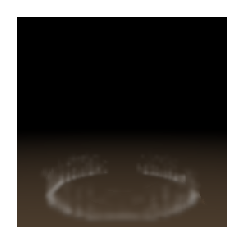
\includegraphics{./img/steam3d-nonoise/render_30.eps}
        \end{center}
        \subcaption{30タイムステップ後}
      \end{minipage}

      % 2
      \begin{minipage}[b]{0.3\linewidth}
        \begin{center}
          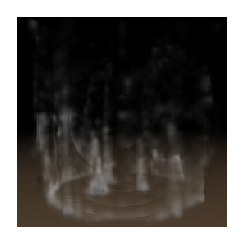
\includegraphics{./img/steam3d-nonoise/render_60.eps}
        \end{center}
        \subcaption{60タイムステップ後}
      \end{minipage}
      
      % 3
      \begin{minipage}[b]{0.3\linewidth}
        \begin{center}
          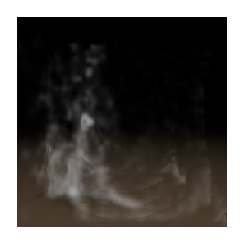
\includegraphics{./img/steam3d-nonoise/render_90.eps}
        \end{center}
        \subcaption{90タイムステップ後}
      \end{minipage}

    \caption{湯気のシミュレーションのレンダリング結果(ノイズがない場合)}
    \label{result-no_noise}
  \end{center}
\end{figure*}

\begin{table}[htb]
  \begin{center}
    \caption{各レンダリング結果のパラメータ}
    \begin{tabular}{|l|c|r||r|} \hline
      パラメータ & 図(\ref{result}) & 図(\ref{result-high_dens}) & 図(\ref{result-high_vapor}) \\ \hline \hline
      密度係数($\rho$) & 1.0 & 5.0 & 1.0 \\      
      浮力係数($k_{b}$) & 1.5 & 1.5 & 1.5 \\
      環境温度($z$) & 1.0 & 1.0 & 0.1 \\
      抗力係数 & 0.07 & 0.07 & 0.07 \\       
      レイノルズ数 & 1.3 & 1.3 & 1.3 \\ 
      浮力係数($k_{b}$) & 1.5 & 1.5 & 1.5 \\
      底辺の温度 & 2.0(ノイズあり) & 2.0(ノイズあり) & 2.0(ノイズあり) \\ 
      底辺の水蒸気量 & 0.5+1.0(ノイズあり) & 0.5+1.0(ノイズあり) & 1.5+1.0(ノイズあり) \\\hline
    \end{tabular}
  \end{center}
\end{table}
\end{comment}

\chapter{結論}

本論文では湯気の物理的な発生原理をもとにしてモデルの構築と実装を行い,湯気の発生する様子をシミュレーションと可視化を行った.
実装においては格子法と粒子法を組み合わせる手法を提案し,湯気の微細な形状の再現を行った.
